% Universidade Federal de Campina Grande
% Proposta de Dissertação de Mestrado em Ciencia da Computacao
%
% Aluno: Ricardo Araújo Santos - ricardo@lsd.ufcg.edu.br - ricardo@dsc.ufcg.edu.br
% Orientadora: Raquel Vigolvino Lopes
% Dezembro de 2010

\documentclass[a4paper,titlepage,12pt]{article}

%language
\usepackage[brazil]{babel}
\usepackage[utf8]{inputenc} % codificar arquivo em UTF-8
\usepackage[T1]{fontenc}

%tabelas
\usepackage{longtable}
\usepackage{colortbl}

%figuras
\usepackage{graphics}

\usepackage{color}
\usepackage{times}
\usepackage{fancyheadings}
\usepackage{fancyvrb}

\usepackage{algorithmic}
\usepackage[nothing]{algorithm}
\usepackage{latexsym}

\usepackage{graphicx,url}

\usepackage[portuguese]{nomencl}


\sloppy

% Estilo e espacamento ----------------------------------------
\newlength{\defbaselineskip}
\setlength{\defbaselineskip}{\baselineskip}
\newcommand{\setlinespacing}[1]
{\setlength{\baselineskip}{#1 \defbaselineskip}}
\newcommand{\bc}{\cellcolor{black}}

\setcounter{topnumber}{2}
\renewcommand{\topfraction}{.7}
\setcounter{bottomnumber}{1}
\renewcommand{\bottomfraction}{.3}
\setcounter{totalnumber}{3}
\renewcommand{\textfraction}{.2}
\renewcommand{\floatpagefraction}{.5}
\setcounter{dbltopnumber}{2}
\renewcommand{\dbltopfraction}{.7}
\renewcommand{\dblfloatpagefraction}{.5}

\oddsidemargin -28pt
\evensidemargin -28pt
\marginparwidth 50pt
\marginparsep 5pt
\topmargin -27pt
\hoffset 15mm
\textheight 237mm
\textwidth 155mm
\renewcommand{\baselinestretch}{1.5}
% ------------------------------------------------------------------------


\renewcommand{\nomname}{Lista de Siglas e Abreviaturas}

\makenomenclature

\begin{document}

% Capa ------------------------------------------------------------------------

\pagestyle{empty}

\begin{center}
{\textbf{\Large \textsc{Universidade Federal de Campina Grande}}}
\end{center}

\begin{center}
\textbf{{\Large \textsc{Centro de Engenharia Elétrica e Informática}}}
\end{center}

\begin{center}
{\large \textsc{\textbf{Curso de Mestrado em Ciência da Computação}}}
\end{center}

~\\ \\

\begin{center}
{\LARGE \textsc{\textbf{Proposta de Dissertação de Mestrado}}}
\end{center}

~\\ \\

\begin{center}
{\Large \textsc{\textbf{Provisão Dinâmica de Recursos Baseada em Métricas de Negócio para Aplicações \textit{SaaS}}}}
%% palavras que deveriam aparecer: automático aplicações SaaS escalonamento (recursos dinâmicos)
\end{center}

~\\ \\

\begin{center}
\textbf{\textsc{Mestrando} \\
\textsc{Ricardo Araújo Santos}}
\end{center}

\begin{center}
\textbf{\textsc{Orientadora} \\
\textsc{Raquel Vigolvino Lopes}}
\end{center}

~\\ \\ \\

\begin{center}
\textbf{{\large \textsc{Campina Grande}}
\\
{\large \textsc{Fevereiro - 2011}}}
\end{center}

\newpage
\cleardoublepage

% ------------------------------------------------------------------------

% Algarismos romanos para as páginas de listagem.
\pagestyle{plain}
\pagenumbering{roman}


\setcounter{page}{2}
\printnomenclature[1cm]

\newpage
\listoffigures

\vspace{3cm}

\listoftables
\newpage

\tableofcontents
\newpage

% Corpo do documento -------------------

% Algarismos arábicos para as páginas do corpo.
\pagestyle{plain}
\pagenumbering{arabic}

%%%%%%%%%%%%%%%%%%%%%%%%%%%%%%%%%%%%%%%%%%%%%%%%%%%%%%%%%%%%%%%%%%%%%%%%%%%%%%%%
% Cabeçalho: secao do lado esquerdo e numero da pagina do lado direito
\pagestyle{fancy}
\addtolength{\headwidth}{\marginparsep}\addtolength{\headwidth}{\marginparwidth}\headwidth
= \textwidth
\renewcommand{\sectionmark}[1]{\markright{\thesection\ #1}}\lhead[\fancyplain{}{\bfseries\thepage}]%
{\fancyplain{}{\emph{\rightmark}}}\rhead[\fancyplain{}{\bfseries\leftmark}]%
{\fancyplain{}{\bfseries\thepage}}\cfoot{}

%%%%%%%%%%%%%%%%%%%%%%%%%%%%%%%%%%%%%%%%%%%%%%%%%%%%%%%%%%%%%%%%%%%%%%%%%%%%%%%%


\setcounter{page}{5}
\section{Introdução}
\label{sec:introducao}

%% Fundamentos (360, berkley)
Nos últimos anos, a computação na nuvem tem modificado vários setores da indústria e academia e, com isso, a ideia de oferecer computação como um serviço utilitário, como energia elétrica, vem se tornando uma realidade. Dessa forma serviços como processamento, armazenamento, infraestrutura ou mesmo o acesso a um software através da internet têm se tornado mais comum tanto para o departamento de Tecnologia da Informação (TI)\nomenclature{TI}{Tecnologia da Informação} das empresas como para os usuários finais. 

%% Subáreas (IaaS, PaaS, SaaS): aprofundar para SaaS
Os serviços oferecidos como computação utilitária abrangem vários níveis, porém não há um consenso na classificação deles. A classificação em ~\cite{cloud-services} é a mais comum na prática e divide os serviços em: (i) Infraestrutura como Serviço (do inglês \textit{Infrastructure as a Service} - \textit{IAAS}\nomenclature{\textit{IAAS}}{\textit{Infrastructure as a Service}}), na qual estão serviços como processamento e armazenamento, tendo como exemplos mais conhecidos o Amazon Elastic Compute Cloud~\cite{amazon-ec2} e GoGrid~\cite{gogrid}; (ii) Plataforma como Serviço (do inglês \textit{Platform as a Service} - \textit{PAAS}\nomenclature{\textit{PAAS}}{\textit{Platform as a Service}}), englobando ferramentas para auxiliar desde o desenvolvimento de aplicações até a manutenção do ciclo de vida delas, representada aqui pelo Google App Engine~\cite{google-appengine}; e (iii) Software como Serviço (do inglês \textit{Software as a Service} - \textit{SAAS}\nomenclature{\textit{SAAS}}{\textit{Software as a Service}}), ofertando aplicações prontas para o usuário final, tendo como exemplos mais conhecidos aplicações para \textit{Customer Relationship Management (CRM)}\nomenclature{\textit{CRM}}{\textit{Customer Relationship Management}} e editores de texto.

\subsection{Características de aplicações SaaS}
%% Software as a Service
%% De onde surgiu a ideia?
A ideia de prover acesso a aplicações por meio de \textit{SaaS} não é nova. Brereton e Budgen~\cite{saas-firstreport} argumentaram em 1999 a favor do desenvolvimento de software em componentes independentes que juntos entregariam um serviço de mais alto nível ao usuário. Já a ideia de separar os papéis de dono e usuário do software é defendida por Turner et al.~\cite{saas-ownership-usage}. Essas duas características ajudam a formar um conceito mais geral de \textit{SaaS} no qual serviços são oferecidos possivelmente por diferentes donos, agregados formando um novo serviço e oferecido ao usuário final que, por sua vez, utiliza o software por meio de uma assinatura e não é responsável por manter o serviço. 

%% Características (Como são as aplicações SaaS?)
Além disso, algumas outras características marcantes de \textit{SaaS} foram identificadas em ~\cite{saas-characteristics} como:

\begin{description}
    \item[Cobrança em um grão pequeno:] 
    As aplicações \textit{on-premise}~\footnote{\textit{on-premise} significa executar a aplicação in loco, na infraestrutura local da empresa, em oposição a \textit{off-premise}, que significa executar numa infraestrutura remota. Aplicações \textit{SaaS} são  comumente chamadas de \textit{off-premise applications}.} possuem um sistema de licença única no momento da aquisição da aplicação. No caso das aplicações \textit{SaaS}, licensas temporárias são adquiridas com base na quantidade de usuários aos quais se quer prover acesso e a cobrança é feita de acordo com a quantidade usada do serviço (processamento utilizado, quantidade de dados armazenados ou transferidos, por exemplo). Dessa forma, tanto o usuário da aplicação acaba por economizar já que a cobrança é mais justa com relação ao tempo de uso da aplicação como o provedor da aplicação lucra provendo uma mesma aplicação para diferentes usuários.  
    \item[Fácil composição de aplicações:] É muito comum utilizar resultados de um serviço como entrada de outros serviços de forma a produzir um serviço mais especializado agregando valor a um ou mais outros. Isso tem sido possível atualmente com a utilização de tecnologias de Arquitetura Orientada a Serviços (do inglês \textit{Service Oriented Architecture - SOA}\nomenclature{\textit{SOA}}{\textit{Service Oriented Architecture}}). Um exemplo pode ser uma aplicação que oferece serviço de edição de texto com correção automática provida por um serviço responsável somente por correção de texto.
    \item[Multi-locação:] Que significa prover acesso a uma mesma aplicação para diferentes usuários de diferentes empresas, impedindo que um acesse informações do outro. Nesse caso, as aplicações podem ser genéricas o suficiente para permitir uma adaptação e customização do serviço oferecido a diferentes clientes. É necessário também uma gerência mais específica dos recursos utilizados para executar as diferentes instâncias do serviço impedindo que o alto processamento solicitado numa instância possa resultar num atraso no tempo de resposta de outra instância.
    \item[Alta escalabilidade:] Durante o desenvolvimento da aplicação, há um esforço por parte dos desenvolvedores para que a aplicação funcione eficientemente ao atender diferentes demandas de usuários.
    \item[Facilidade de disponibilizar a aplicação na infraestrutura da empresa:] Como o serviço é acessado através da internet, mudar a infraestrutura onde a aplicação está hospedada não deve ser uma tarefa difícil. Dessa forma, uma empresa pode utilizar recursos próprios disponíveis para executar a aplicação e em momentos de sobrecarga de requisições balancear a carga executando novas instâncias da aplicação em infraestruturas remotas.
    \item[Internacionalização:] Disponibilizar a aplicação para usuários acessando a partir de diferentes regiões geográficas. Isso pode requerer uma adaptação do serviço ao idioma nativo do cliente e sistemas de medida e moedas diferentes, como também a personalização do próprio servido. Como exemplo disso, pode-se pensar num sistema de busca por restaurantes que ofereçe resultados diferentes dependendo da região geográfica a partir da qual a requisição foi originada. Essa preocupação surge ainda durante o design da aplicação.
\end{description}

\subsection{Vantagens da metodologia \textit{SaaS}}

Muitas são as vantagens desse modelo de entrega de serviço, tanto para o usuário final como para quem provê o serviço. Do lado de quem usa, as pequenas e médias empresas têm seus custos reduzidos com o uso do modelo \textit{pay-as-you-go} pois não há mais a necessidade de adquirir e manter a aplicação muito menos infraestrutura para sua execução~\cite{saas-small-medium-enterprise}. Grandes empresas, por usa vez, tiram proveito do fato de não precisar desenvolver uma nova aplicação. Além disso, há também a possibilidade de executar na própria infraestrutura da empresa reduzindo preocupações com segurança de dados críticos.

Na academia, iniciativas como Globus Online~\cite{globus-online} e R-PHP~\cite{r-php} mostram a viabilidade na utilização desse modelo para prover serviços que auxiliem os pesquisadores durante o ciclo da pesquisa. Serviços como edição de texto, processadores de dados, classificação de artigos são de interesse de muitos pesquisadores e o uso de ferramentas que não necessitem de instalação reduz bastante o trabalho adicional e permitem um maior foco no próprio processo da pesquisa.

Quanto aos provedores, a mesma aplicação pode ser provida a vários usuários de empresas diferentes. Dessa forma, custos com manutenção da aplicação e infraestrutura são compensados com a economia de escala já que a mesma infraestrutura pode ser utilizada para manter o mesmo serviço para milhares de clientes independentes. No entanto vários outros problemas surgem com o emprego desse modelo: (i) preocupações com a modelagem, design, construção e manutenção de aplicações SaaS, tem sido um alvo de trabalhos como ~\cite{software-modeling,software-development}; (ii) segurança privacidade de dados críticos de empresas; (iii) como prover internacionalização; (iv) como fazer balanceamento de carga entre servidores; entre muitos outros. 

\subsection{Provisão de Recursos}

Um problema interessante e que merece uma atenção especial por impactar diretamente nos lucros do provedor diz respeito a como o provedor executa a aplicação. A figura \ref{figura:saas-layers} mostra como os diferentes papéis interagem nesse processo. Clientes usam os serviços disponibilizados pelo provedor de \textit{SaaS} que, por sua vez, adquire recursos de um ou mais provedores de \textit{PaaS} ou diretamente de provedores de \textit{IaaS}. Tanto a forma com a qual esses recursos são adquiridos como a forma como são utilizados impactam diretamente no custo de manter os serviços e, consequentemente, no lucro do provedor. 

\begin{figure}[htp]
\begin{center}
  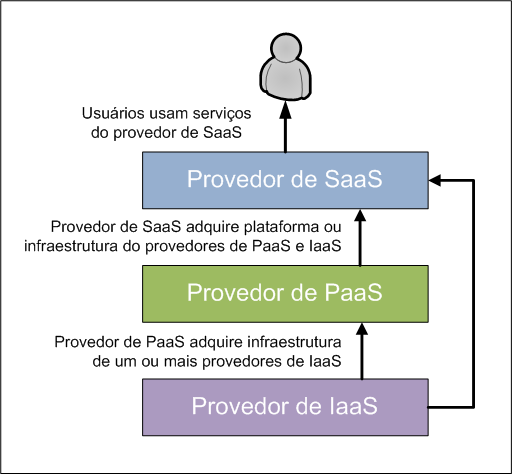
\includegraphics[width=0.5\textwidth]{figures/saas-layers.png}
  \caption[Interação entre clientes e provedores]{Interação entre clientes e provedores}
  \label{figura:saas-layers}
\end{center}
\end{figure}

Atualmente, o provedor de \textit{IaaS} mais conhecido é o Amazon EC2~\cite{amazon-ec2}. Diversos tipos de máquinas virtuais são oferecidos a preços diferentes. O usuário paga pelo tempo que usa, pela quantidade de dados transferida e armazenada nas instâncias. Existem três formas de aquisição de máquinas virtuais~\cite{amazon-pricing}:

\begin{description}
  	\item [Mercado sob demanda:] As máquinas são compradas sem a necessidade de um contrato ou reserva. Dessa forma o usuário pode facilmente aumentar e diminuir a capacidade da aplicação. Em momentos de sobrecarga, pode ser que a Amazon não tenha máquinas para oferecer e, portanto, o pedido de aquisição de instâncias sob demanda ser negado;
    \item [Mercado de reserva:] Nessa modalidade as máquinas são reservadas pelo intervalo de 1 a 3 anos a um preço mais baixo que o do mercado sob demanda. Dessa forma, quando o usuário precisar usar uma máquina reservada, a quantia paga pela hora utilizada é inferior ao do mercado sob demanda. Existe aqui a garantia de que as máquinas reservadas vão estar disponíveis quando solicitadas para uso.  
  	\item [Mercado baseado em lances de oferta:] Essa modalidade de mercado é adequada para quem precisa de máquinas num grão menor que o do mercado sob demanda. O usuário especifica um preço limite para a máquina-hora. Como o preço da instância flutua baseado na oferta e demanda por máquinas desse tipo, quando o preço da instância está abaixo do limite especificado pelo usuário, a máquina é vendida. Se o preço da instância ultrapassar o limite do usuário, a máquina é encerrada.
\end{description}   

Dessa forma um provedor pode, por exemplo, planejar um ano de utilização de recursos reservando instâncias no mercado de reserva, atender picos de requisições com instâncias sob demanda e reduzir custos comprando máquinas no mercado baseado em lances. Nesse caso, problemas interessantes surgem no momento de escalonar a aplicação na infraestrutura disponível no momento, mesmo não havendo um planejamento a ser seguido.

Alguns objetivos, não mutuamente excludentes, de quem é responsável por escalonar a aplicação na infraestrutura são: (i) maximizar o número de usuários atendidos; (ii) assegurar que os Acordos de Nível de Serviço (do inglês \textit{Service Level Agreement - SLA}\nomenclature{\textit{SLA}}{\textit{Service Level Agreement}}) com os clientes estão sendo mantidos; e (iii) minimizar os custos com a execução da aplicação. 

O problema de provisão de recursos não é novidade na comunidade acadêmica muito menos no departamento de TI das empresas. Urgaonkar et al. ~\cite{multitier}, trata desse problema para aplicações Web multicamadas, enquanto em ~\cite{sla} o escalonamento de aplicações web simples é otimizado com foco no \textit{SLA} estabelecido com o usuário, levando-se em consideração picos de demanda. No campo das aplicações de e-ciência, Kim et al.~\cite{kim-responsetime} otimizam o escalonamento de aplicações com base no tempo de resposta. 

Essas abordagens possuem um ponto em comum, usam métricas muito técnicas e que nem sempre são conhecimento comum de quem é responsável por essa tarefa. Ou ainda, as ferramentas propostas precisam de que o usuário configure certos parâmetros com uma certa acurácia para produzir bons resultados. Visando facilitar mais essa tomada de decisão, o primeiro ponto é o uso de técnicas baseadas em métricas de negócio. Com isso o conhecimento fica mais acessível a quem é responsável pela tomada de decisão no provedor. Naturalmente as métricas mais técnicas serão levadas em consideração, porém acima deste sistema baseado em métricas técnicas estará o sistema baseado em métricas de negócio que irá avaliar diferentes configurações à luz dessas métricas identificando a que trouxer maior retorno para o negócio. O segundo ponto é tornar essa decisão o mais automatizada possível, ou prover uma configuração inicial que permita o uso dessa abordagem sem a necessidade de configurar inicialmente parâmetros sensíveis com tamanha acurácia. 

Pretende-se construir um escalonador de aplicações \textit{SaaS} baseado em métricas de negócio que venha a tirar proveito desse tipo de métrica para reduzir os custos do provedor sem comprometer o serviço oferecido. Inicialmente é necessário capturar características dessas aplicações que possam ser usadas na construção do modelo. A partir disso, é necessária uma forma de valorar essas características capturadas e uma maneira bastante comum é o uso de funções de utilidade. Essa funções mapeiam o valor que os usuários atribuem a execução de aplicações~\cite{wilkes-utility}, podendo ser definidas em termos de tempo de execução, por exemplo. A forma da curva de utilidade, no entanto, depende dos objetivos dos usuários~\cite{lee-utility}. Em se tratando de aplicações Web, como são todas as aplicações \textit{SaaS}, não existe um tempo delimitado de execução da aplicação. A aplicação é de fato um serviço, que está sempre à espera de requisições vindas de diferentes usuários. Um novo modelo que capture esta característica de serviço além dos objetivos dos usuários deve ser criado.

Uma vez caracterizadas as aplicações \textit{SaaS} e seu modelo de valoração, escalonadores cientes dessas métricas de negócio podem tirar proveito dependendo do objetivo escolhido: reduzir custo, reduzir tamanho de fila de espera, aumentar número de requisições atendidas por segundo, por exemplo. Para isso, pretende-se avaliar o desempenho de diferentes heurísticas em diversas situações, inclusive comparando com outras alternativas que tenhas sido encontradas na literatura. 


%%%%%%%%%%%%%%%%%%%%%%%%%%%%%%%%%%%%%%%%%%%%%%%%%%%%%%%%%%%%%%%%%%%%%%%%%%%%%%%%%%%%%%%%%

% \begin{itemize}
%     \item Cloud Computing
%     \begin{itemize}
%         \item Fundamentos (360, berkley)
%         \item Subáreas (IaaS, PaaS, SaaS): aprofundar para SaaS
%     \end{itemize}
%     \item Software as a Service
%     \begin{itemize}
%         \item De onde surgiu a ideia?
%         \item Características (Como são as aplicações SaaS?)
%         \begin{itemize}
%             \item Multi-locação
%             \item Cobrança em um grão pequeno
%             \item Alta escalabilidade
%             \item Fácil composição de aplicações
%             \item Facilidade de disponibilizar a aplicação na infraestrutura interna da empresa
%             \item Internacionalização  
%         \end{itemize}
%         \item Quem tira proveito dessa ideia? (talvez seja melhor isso vir antes de ``Características'')
%         \begin{itemize}
%             \item Pequenas e médias empresas que tem seus custos com software barateados
%             \item Grandes empresas que precisam do serviço imediatamente
%             \item Meio acadêmico com a difusão de softwares de auxilio ao ciclo da pesquisa
%             \item Provedores de SaaS oferecem o mesmo serviço a múltiplos clientes ganhando na economia de escala
%         \end{itemize}
%         \item Quais as dificuldades desse pessoal?
%         \begin{itemize}
%             \item Design, construção e manutenção de aplicações.
%             \item Segurança e privacidade de dados críticos da empresa
%             \item Atendimento de picos de demanda dos usuários
%             \item Prover o mesmo serviço a clientes em diferentes regiões geográficas
%             \item Prover diferentes aplicações numa mesma estrutura e priorizar recursos entre elas
%             \item Usar diferentes infraestruturas para executar a aplicação
%         \end{itemize}
%     \end{itemize}
%     \item Gerência automatizada
%     \begin{itemize}
%         \item Por que é necessária?
%         \begin{itemize}
%             \item O que se ganha?
%             \item O que se perde?
%         \end{itemize}
%         \item Quais as técnicas mais comuns?
%         \begin{itemize}
%             \item Técnicas preditivas
%             \item Técnicas reativas
%             \item Híbridas?
%         \end{itemize}
%     \end{itemize}
%     \item Alguém já tentou fazer gerência automatizada de aplicações SaaS
%     \begin{itemize}
%         \item O que tentaram?
%         \item Resolveu o problema? Por que?
%         \item Qual a ideia que está sendo proposta?
%         \item Existe algum indício de que essa ideia pode ser bem sucedida?
%         \item Os clientes dessa ideia poderão tirar proveitos práticos dela?
%     \end{itemize}
% \end{itemize}

\newpage
\section{Objetivo da Proposta}
\label{sec:objetivo}

O objetivo principal dessa pesquisa é: \textbf{Investigar a viabilidade do uso de técnicas dirigidas por métricas de negócio para a provisão dinâmica de recursos para execução de aplicações \textit{SaaS}.}

Para cumprir esse objetivo, é necessário atingir alguns objetivos secundários:

\begin{itemize}
  \item Capturar características importantes das aplicações em estudo para que o modelo construído possa tirar proveito dessas especialidades;
  \item Criar e avaliar um modelo de escalonador que automatize a alocação de recursos;
  \item Traçar conclusões gerais a respeito do modelo para que ele não seja útil somente nos cenários avaliados. 
\end{itemize}

\section{Relevância da Proposta}
\label{sec:relev}

O uso de aplicações \textit{SaaS} está cada vez mais comum nas empresas assim como a academia também tem como tirar proveito desse modelo. Espera-se apontar novos caminhos na área de provisão dinâmica de recursos para esse tipo de aplicação e a sugestão ou amadurecimento de métricas de negócio, bem como a proposta de um escalonador que possa automatizar essa atividade.

Com o sucesso dessa pesquisa, provedores de \textit{SaaS} poderão tirar um melhor proveito de sua infraestrutura local ou da infraestrutura adquirida em outros provedores fazendo um uso mais eficiente dos recursos atendendo à demanda dos usuários da aplicação. O uso de métricas de negócio torna mais simples a gerência da aplicação uma vez que os resultados de uma decisão refletem diretamente em métricas compreensíveis por quem tem o poder de decisão na empresa. Uma vez bem estudadas e documentadas, essa métricas podem, além de guiar o processo de tomada de decisão, atuar na automação desse processo.

% \begin{itemize}
%     \item Quem ganha com o sucesso do meu trabalho?
%     \begin{itemize}
%         \item Provedor de SaaS que quer tirar um melhor proveito da sua infraestrutura local assim como fazer um melhor uso de recursos adquiridos em provedores de PaaS e IaaS.
%         \item Tornar a tomada de decisão sobre a aplicação mais fácil para o gerente com o uso de uma abordagem dirigida a negócio.
%     \end{itemize}
%     \item Que contribuições eu espero atingir com a finalização da pesquisa?
%     \begin{itemize}
%         \item Apontar caminhos na área de provisão dinâmica de recursos para esse tipo de aplicação
%         \item Propor métricas de negócio para simplificar a vida de quem oferece esse tipo de aplicação
%         \item Apresentar heurísticas que realizem esse trabalho de uma forma mais simples/eficiente do que se tem encontrado na literatura.
%     \end{itemize}
% \end{itemize}

\newpage
\section{Metodologia de Trabalho}
\label{sec:metodologia}

Através dos objetivos levantados na seção \ref{sec:objetivo}, algumas atividades foram elencadas para o sucesso da pesquisa. Essas atividades estão resumidas na tabela \ref{table:atividades} e abaixo segue uma descrição detalhada de cada atividade e dos resultados esperados. O cronograma planejado é apresentado na subseção \ref{cronograma}.

\begin{table}[H]
\centering
\begin{tabular}{|c|p{0.8\textwidth}|}
    \hline
Atividades & \multicolumn{1}{c}{Descrição}\\
	\hline
A1 & Levantamento bibliográfico sobre caracterização e valoração de aplicações \textit{SaaS}\\
	\hline
A2 & Caracterização de aplicações \textit{SaaS}\\
	\hline
A3 & Elaborar um modelo de valoração de aplicações \textit{SaaS}\\
	\hline
A4 & Levantamento bibliográfico sobre provisão dinâmica de recursos, apoiadas em métricas de negócio, para aplicações \textit{SaaS}\\
	\hline
A5 & Elaboração de heurísticas para provisão dinâmica de recursos para aplicações \textit{SaaS}\\
	\hline
A6 & Avaliação das heurísticas propostas\\
	\hline
A7 & Escrita da dissertação\\
	\hline
A8 & Escrita de um artigo para uma conferência internacional ou periódico\\
	\hline
A9 & Defesa da dissertação\\
	\hline
\end{tabular}
\caption{Atividades Planejadas}
\label{table:atividades}
\end{table}

\subsection*{A1 - Levantamento bibliográfico sobre caracterização e valoração de aplicações \textit{SaaS}}
Essa atividade é fundamental para se ter conhecimento do estado da arte da área. Esse levantamento bibliográfico é fundamental e mais demorado no início da pesquisa mas é retomado a cada ciclo completo da pesquisa. Com isso a revisão da área não fica desatualizada. Essa atividade tem como resultados: (i) parte da seção de trabalhos relacionados da dissertação e do artigo científico; (ii) conhecimento para auxílio nas atividades A2 e A3.

\subsection*{A2 - Caracterização de aplicações \textit{SaaS}}
Com base no primeiro levantamento bibliográfico feito, dá-se início ao processo de caracterização de aplicações \textit{SaaS}. Essa atividade tem como resultado a documentação de características importantes a serem levadas em conta na elaboração do modelo de valoração. Essa atividade também pode vir a reduzir o escopo de alcance do trabalho e a pesquisa se focar nas classes mais representativas de aplicações encontradas.

\subsection*{A3 - Elaborar um modelo de valoração de aplicações \textit{SaaS}}
Como o foco do trabalho reside nas métricas de negócio, essa atividade usa o conhecimento coletado na atividade A1 e A2 na construção de um modelo que leve em conta as características levantadas. Um modelo já existente pode ser usado, ou ainda, aperfeiçoado. Um objetivo importante dessa fase está na identificação das métricas de negócio que serão alvo na fase de avaliação do escalonador. O resultado dessa fase é um modelo de valoração de aplicações \textit{SaaS} com base em métricas de negócio identificadas.

\subsection*{A4 - Levantamento bibliográfico sobre provisão dinâmica de recursos, apoiadas em métricas de negócio, para aplicações \textit{SaaS}}
Essa atividade dá início a linha principal da pesquisa. Com essa revisão, será possível identificar escalonadores/heurísticas/algoritmos para provisão dinâmica que possam ser usados para comparação com as heurísticas propostas. É desejável que os algoritmos usados na comparação sejam baseados em métricas de negócio também. Essa atividade tem como resultados: (i) parte da seção de trabalhos relacionados da dissertação e do artigo; (ii) uma fundamentação para a análise do escalonador proposto; e (iii) uma formulação matemática do problema analisado.

\subsection*{A5 - Elaboração de heurísticas para provisão dinâmica de recursos para aplicações \textit{SaaS}}
Uma vez modelada a valoração das aplicações, essa atividade tem por finalidade completar essa modelagem propondo um novo escalonador baseado nas métricas de negócio modeladas. Espera-se levantar várias propostas de heurística que considerem situações diferentes ou que priorizem métricas diferentes. Os resultados dessa atividade são: (i) uma modelagem analítica de um escalonador baseado em métricas de negócio; (ii) um simulador desse escalonador proposto; (iii) uma modelagem analítica de uma ou mais heurísticas; e (iv) implementações dessas heurísticas para serem avaliadas no simulador. 

\subsection*{A6 - Avaliação das heurísticas propostas}
Com uma modelagem do problema e das heurísticas é possível tirar conclusões através de uma avaliação analítica de situações bem conhecidas. Essas conclusões podem ser usadas no processo de verificação do modelo de simulação. Com um modelo de simulação implementado, novas situações podem ser analisadas e conclusões mais gerais sobre a solução podem ser traçadas. Nesse caso, deve ser feito antes de cada seção de experimentação um design do experimento com a finalidade de guiar o processo de seleção de fatores e tratamentos importantes para serem analisados. Os resultados dessa atividade são: (i) a seção de modelagem e análise de resultados da dissertação e do artigo científico. As conclusões extraídas dessa análise podem requerer um refinamento do modelo e portanto um retorno às atividades anteriores. 

\subsection*{A7 - Escrita da dissertação}
Essa atividade será realizada durante todo o processo da pesquisa documentando os resultados de todas as outras atividades.

\subsection*{A8 - Escrita de um artigo para uma conferência internacional ou periódico}
No final dos últimos ciclos da pesquisa (estudo - modelagem - avaliação), será estudada a possibilidade de publicação das conclusões extraídas dos resultados parciais do trabalho numa conferência internacional ou periódico. O resultado dessa atividade é a publicação dos resultados na comunidade internacional.

\subsection*{A9 - Defesa da dissertação}
Essa atividade põe fim ao ciclo dessa pesquisa, apresentando os resultados a comunidade científica e contribuindo com o estado da arte da área pesquisada. 

\newpage
\subsection{Cronograma}
\label{cronograma}

%%\usepackage{colortbl} incluir para colorir as células.

O planejamento de execução das atividades identificadas na tabela~\ref{table:atividades} está representado na tabela~\ref{table:cronograma}. 

\begin{table}[H]
\centering
\begin{tabular}{|c|c|c|c|c|c|c|c|c|c|c|c|c|c|c|c|c|c|c|c|c|c|c|c|c|}
    \hline
 & \multicolumn{4}{c|}{Mar/2011} & \multicolumn{4}{c|}{Abr/2011} & \multicolumn{4}{c|}{Mai/2011} & \multicolumn{4}{c|}{Jun/2011} & \multicolumn{4}{c|}{Jul/2011} & \multicolumn{4}{c|}{Ago/2011}\\    
	\hline
A1 & \bc & \bc & \bc & \bc & \bc & \bc & \bc & \bc &     &     &     &     &     &     &     &     &     &     &     &     &     &     &     &\\
	\hline
A2 &     &     &     &     & \bc & \bc & \bc & \bc &     &     &     &     &     &     &     &     &     & \bc & \bc & \bc &     &     &     &\\
	\hline
A3 &     &     &     &     &     &     &     & \bc & \bc & \bc & \bc & \bc &     &     &     &     &     & \bc & \bc & \bc &     &     &     &\\
	\hline
A4 &     &     &     &     &     &     &     &     &     &     & \bc & \bc & \bc & \bc &     &     &     &     & \bc & \bc & \bc & \bc &     &\\
	\hline
A5 &     &     &     &     &     &     &     &     &     &     &     &     & \bc & \bc & \bc &     &     &     &     &     & \bc & \bc & \bc &\\
	\hline
A6 &     &     &     &     &     &     &     &     &     &     &     &     &     &     & \bc & \bc & \bc & \bc &     &     &     &     & \bc & \bc\\
	\hline
A7 & \bc & \bc & \bc & \bc & \bc & \bc & \bc & \bc & \bc & \bc & \bc & \bc & \bc & \bc & \bc & \bc & \bc & \bc & \bc & \bc & \bc & \bc & \bc & \bc\\
    \hline
A8 &     &     &     &     &     &     &     &     &     &     &     &     &     &     &     &     &     &     &     &     &     &     &     &\\
    \hline
A9 &     &     &     &     &     &     &     &     &     &     &     &     &     &     &     &     &     &     &     &     &     &     &     &\\
    \hline
 & \multicolumn{4}{c|}{Set/2011} & \multicolumn{4}{c|}{Out/2011} & \multicolumn{4}{c|}{Nov/2011} & \multicolumn{4}{c|}{Dez/2011} & \multicolumn{4}{c|}{Jan/2012} & \multicolumn{4}{c|}{Fev/2012}\\    
	\hline
A1 &     &     &     &     &     &     &     &     &     &     &     &     &     &     &     &     &     &     &     &     &     &     &     &\\
	\hline
A2 &     & \bc & \bc & \bc &     &     &     &     &     & \bc & \bc &     &     &     &     &     &     &     &     &     &     &     &     &\\
	\hline
A3 &     & \bc & \bc & \bc &     &     &     &     &     & \bc & \bc &     &     &     &     &     &     &     &     &     &     &     &     &\\
	\hline
A4 &     &     & \bc & \bc & \bc &     &     &     &     &     & \bc & \bc & \bc &     &     &     &     &     &     &     &     &     &     &\\
	\hline
A5 &     &     &     & \bc & \bc & \bc &     &     &     &     &     & \bc & \bc & \bc & \bc &     &     &     &     &     &     &     &     &\\
	\hline
A6 & \bc & \bc &     &     &     & \bc & \bc & \bc & \bc & \bc & \bc &     &     & \bc & \bc & \bc & \bc & \bc & \bc &     &     &     &     &\\
	\hline
A7 & \bc & \bc & \bc & \bc & \bc & \bc & \bc & \bc & \bc & \bc & \bc & \bc & \bc & \bc & \bc & \bc & \bc & \bc & \bc & \bc & \bc & \bc & \bc & \bc\\
A8 &     &     &     &     &     &     &     &     &     & \bc & \bc & \bc & \bc &     &     &     &     &     &     &     &     &     &     &\\
    \hline
A9 &     &     &     &     &     &     &     &     &     &     &     &     &     &     &     &     &     &     &     &     &     &     &     & \bc\\
    \hline
\multicolumn{1}{c}{\rule{0.3cm}{0cm}} &
\multicolumn{1}{c}{\rule{0.1cm}{0cm}} &
\multicolumn{1}{c}{\rule{0.1cm}{0cm}} &
\multicolumn{1}{c}{\rule{0.1cm}{0cm}} &
\multicolumn{1}{c}{\rule{0.1cm}{0cm}} &
\multicolumn{1}{c}{\rule{0.1cm}{0cm}} &
\multicolumn{1}{c}{\rule{0.1cm}{0cm}} &
\multicolumn{1}{c}{\rule{0.1cm}{0cm}} &
\multicolumn{1}{c}{\rule{0.1cm}{0cm}} &
\multicolumn{1}{c}{\rule{0.1cm}{0cm}} &
\multicolumn{1}{c}{\rule{0.1cm}{0cm}} &
\multicolumn{1}{c}{\rule{0.1cm}{0cm}} &
\multicolumn{1}{c}{\rule{0.1cm}{0cm}} &
\multicolumn{1}{c}{\rule{0.1cm}{0cm}} &
\multicolumn{1}{c}{\rule{0.1cm}{0cm}} &
\multicolumn{1}{c}{\rule{0.1cm}{0cm}} &
\multicolumn{1}{c}{\rule{0.1cm}{0cm}} &
\multicolumn{1}{c}{\rule{0.1cm}{0cm}} &
\multicolumn{1}{c}{\rule{0.1cm}{0cm}} &
\multicolumn{1}{c}{\rule{0.1cm}{0cm}} &
\multicolumn{1}{c}{\rule{0.1cm}{0cm}} &
\multicolumn{1}{c}{\rule{0.1cm}{0cm}} &
\multicolumn{1}{c}{\rule{0.1cm}{0cm}} &
\multicolumn{1}{c}{\rule{0.1cm}{0cm}} \\
\end{tabular}
\caption{Cronograma}
\label{table:cronograma}
\end{table}


\newpage

%% Bibliografia ----------------------------------------------------------------
\bibliographystyle{alpha} % estilo de bibliografia
\bibliography{proposta} % arquivos com as entradas bib.

\end{document}
